\chapter{Results}

\section{Application Functionality Overview}
The completed SmartLib desktop system successfully unifies core library circulation operations into a cohesive graphical user interface. The system provides responsive navigation between administrative tasks for librarians and self-service inquiries for students.

Key operational capabilities verified in the live system include:
\begin{itemize}
    \item \textbf{Dual Portal Navigation:} An ergonomic login portal allowing librarians to authenticate with administrative credentials and students to authenticate via their KTU registration identifiers.
    \item \textbf{Analytical Oversight:} Real-time executive dashboards aggregating key operational metrics (collection size, active loan counts, overdue books, and most frequently checked-out literature).
    \item \textbf{Dynamic Circulation Desk:} A live 10-column tracking interface displaying all currently active borrowings, computing clock-aware overdue days and monetary fines on the fly ($\text{\rupee} 10.00$/day), and supporting immediate one-click returns.
    \item \textbf{FIFO Reservation Queue:} Title-level reservations that automatically prompt circulation staff when matching physical copies are returned.
    \item \textbf{Student Self-Service:} Direct book catalog exploration, digital borrow requests, and real-time loan status transparency.
\end{itemize}

\section{User Interface Walkthrough and Screenshots}

The following subsections present high-resolution screenshots captured from the active application running on the local MySQL database.

\subsection{User Authentication and Registration Portal}
Figure~\ref{fig:screenshot_login} displays the primary entry point to SmartLib. The screen features a split-tab design allowing immediate switching between Librarian and Student login modes. Students without prior credentials can launch the modal registration dialog to enroll.

\begin{figure}[h!]
    \centering
    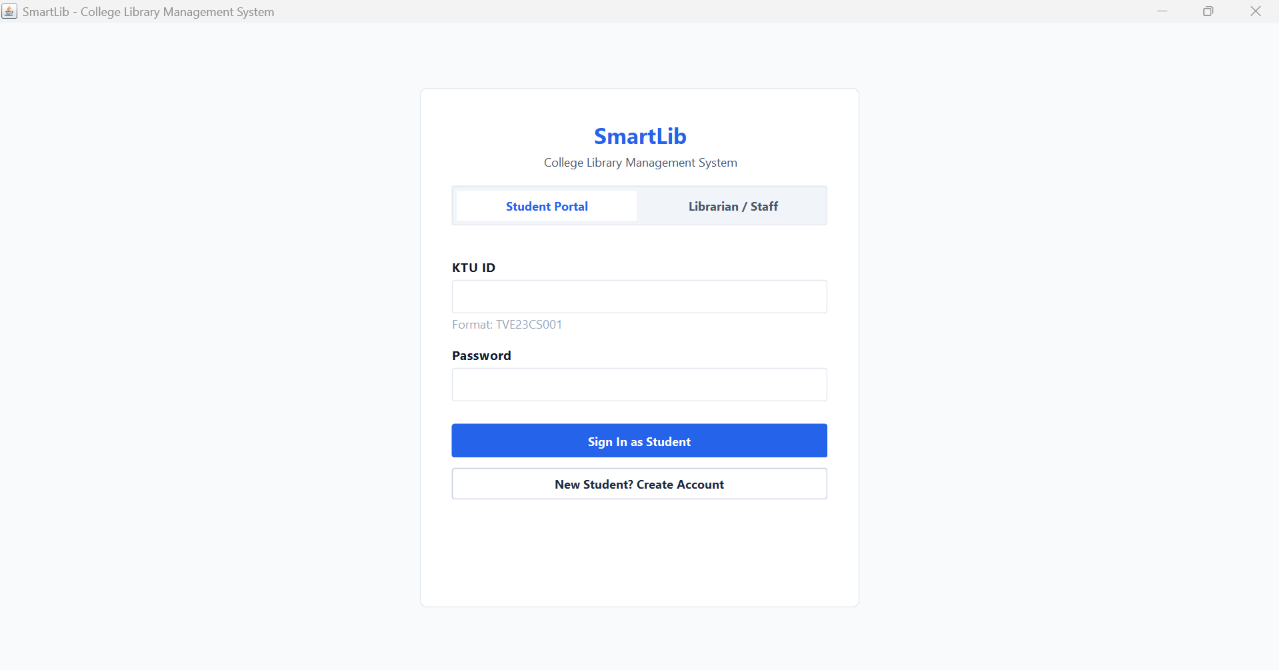
\includegraphics[width=0.94\textwidth]{figures/auth.png}
    \caption{SmartLib User Authentication Portal (\texttt{LoginPanel})}
    \label{fig:screenshot_login}
\end{figure}

\subsection{Executive Analytics Dashboard}
Figure~\ref{fig:screenshot_dashboard} illustrates the Librarian Dashboard. Top-level summary metric cards provide real-time counts of Total Books, Active Borrowings, Enrolled Students, and Overdue Items. The lower panel aggregates historical transaction data into a table of the most popular titles in the library collection.

\begin{figure}[h!]
    \centering
    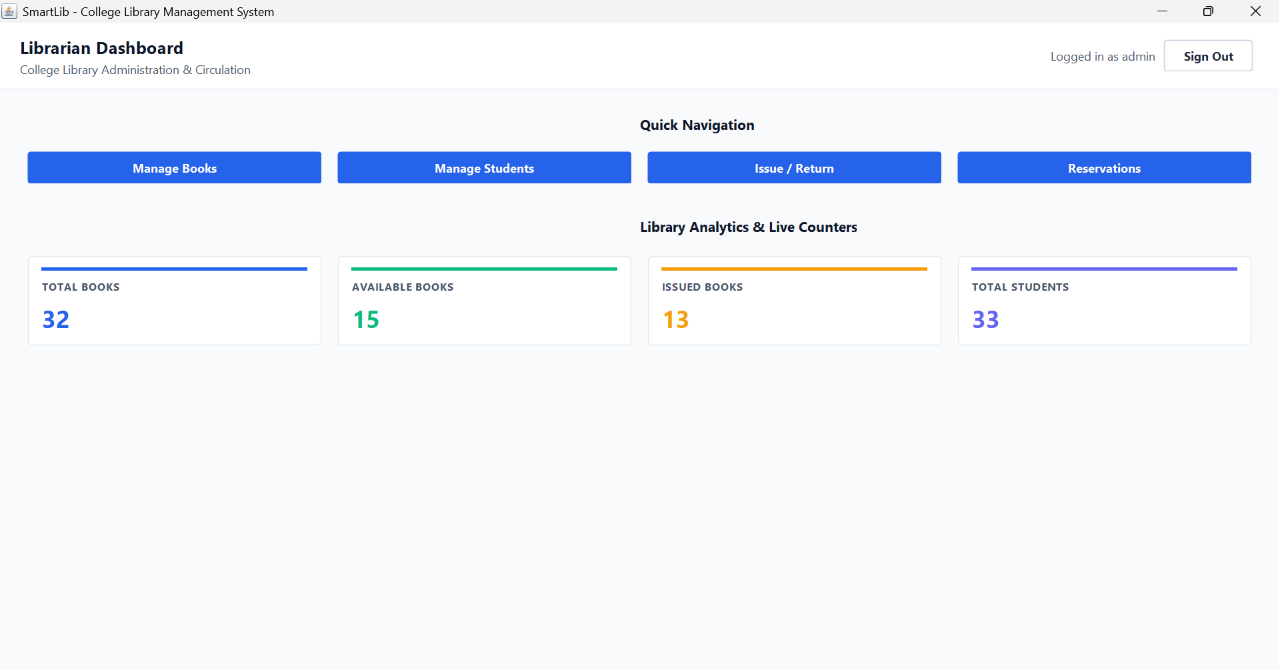
\includegraphics[width=0.94\textwidth]{figures/librarian-dashboard.png}
    \caption{Librarian Executive Analytics Dashboard (\texttt{DashboardPanel})}
    \label{fig:screenshot_dashboard}
\end{figure}

\subsection{Book Inventory Management Panel}
Figure~\ref{fig:screenshot_books} depicts the Book Catalog management interface. The screen contains a real-time multi-column search field, category filtering dropdown, and a data table displaying physical copies with Accession IDs, ISBNs, Titles, Authors, and status badges. The action header allows librarians to add new book copies or delete selected entries (in-place metadata editing is not included in the current UI version).

\begin{figure}[h!]
    \centering
    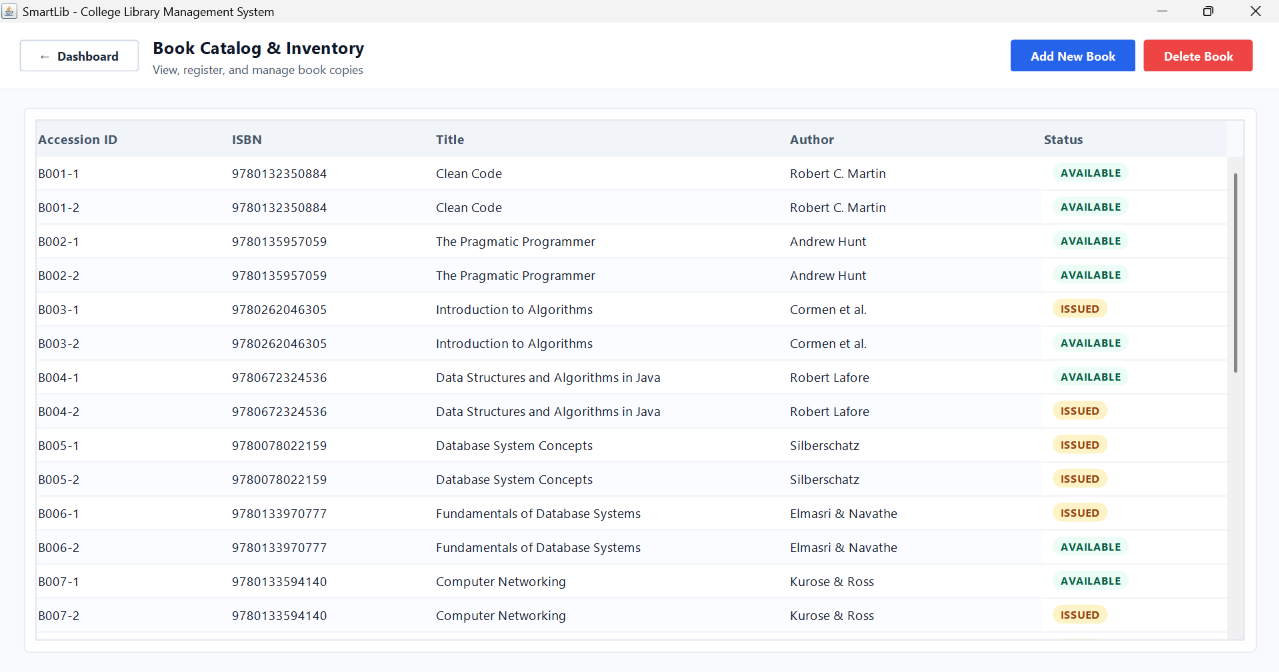
\includegraphics[width=0.94\textwidth]{figures/book-inventory-librarian.png}
    \caption{Book Catalog and Inventory Management Panel (\texttt{BookPanel})}
    \label{fig:screenshot_books}
\end{figure}

\subsection{Student Directory and Account Management Panel}
Figure~\ref{fig:screenshot_students} shows the Student Directory desk. Entering a valid KTU ID during student registration automatically parses and populates the student's admission year, batch, and engineering branch. The panel allows librarians to view registered student profiles, activate or deactivate circulation access, and delete accounts (subject to deletion safeguards preventing removal of students with active loans or unreturned records).

\begin{figure}[h!]
    \centering
    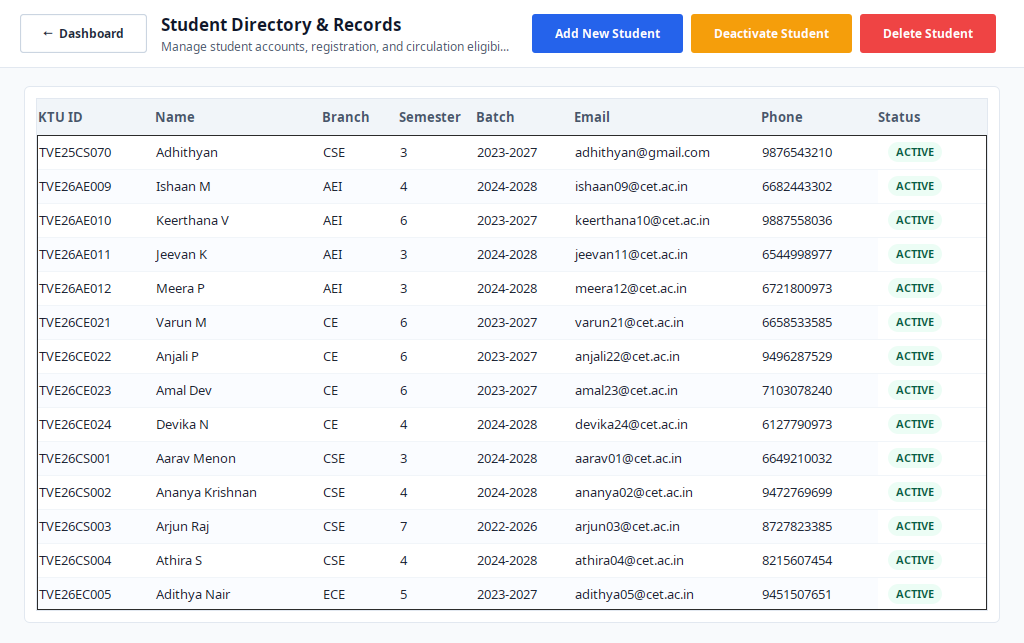
\includegraphics[width=0.94\textwidth]{figures/screenshot_students.png}
    \caption{Student Directory and Account Management Panel (\texttt{StudentPanel})}
    \label{fig:screenshot_students}
\end{figure}

\subsection{Circulation Desk and Active Borrowings Panel}
Figure~\ref{fig:screenshot_borrow} illustrates the core Circulation Desk. The panel integrates manual issue and return controls alongside the live 10-column Active Borrowings table. Librarians can apply status filters (\texttt{All Active}, \texttt{Overdue}, \texttt{Due Today}), search by student name or book title, observe live overdue calculations, and execute direct returns from selected rows.

\begin{figure}[h!]
    \centering
    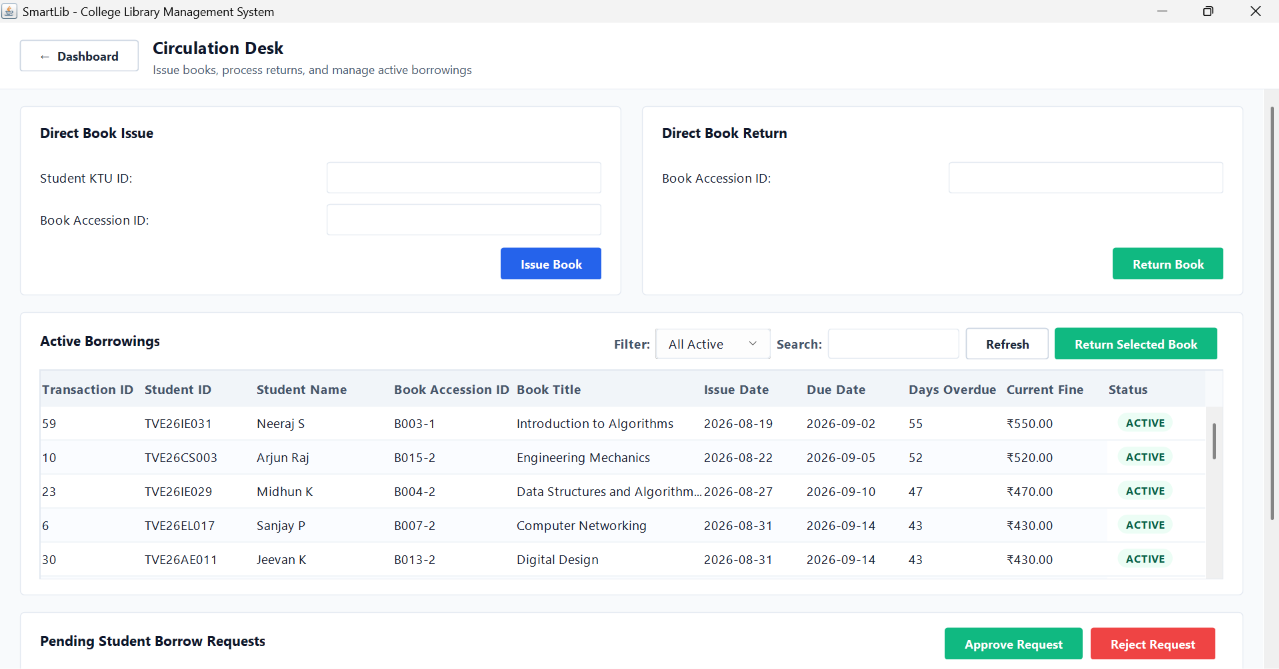
\includegraphics[width=0.94\textwidth]{figures/borrow-management.png}
    \caption{Circulation Desk and Active Borrowings Management Panel (\texttt{BorrowPanel})}
    \label{fig:screenshot_borrow}
\end{figure}

\subsection{Reservation Queue Management Panel}
Figure~\ref{fig:screenshot_reservation} displays the Title Reservation desk. Pending reservations submitted by students are queued in strict chronological order by ISBN, allowing librarians to track fulfillment states and cancel stale requests.

\begin{figure}[h!]
    \centering
    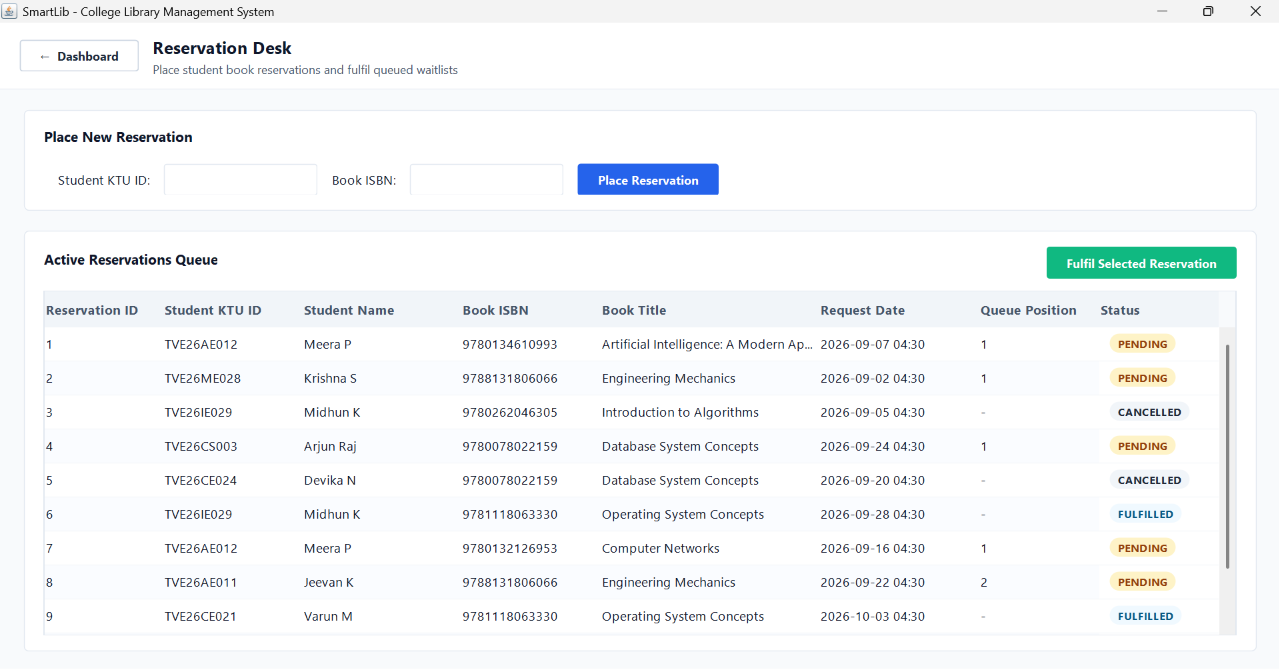
\includegraphics[width=0.94\textwidth]{figures/reservation-queue-list.png}
    \caption{Title Reservation Queue Management Panel (\texttt{ReservationPanel})}
    \label{fig:screenshot_reservation}
\end{figure}

\subsection{Student Self-Service Dashboard}
Figure~\ref{fig:screenshot_student_dashboard} depicts the student portal view. Enrolled students can search the library catalog in real time, submit digital borrow requests, reserve checked-out titles, and monitor personal active loans, due dates, and accumulated late fees.

\begin{figure}[h!]
    \centering
    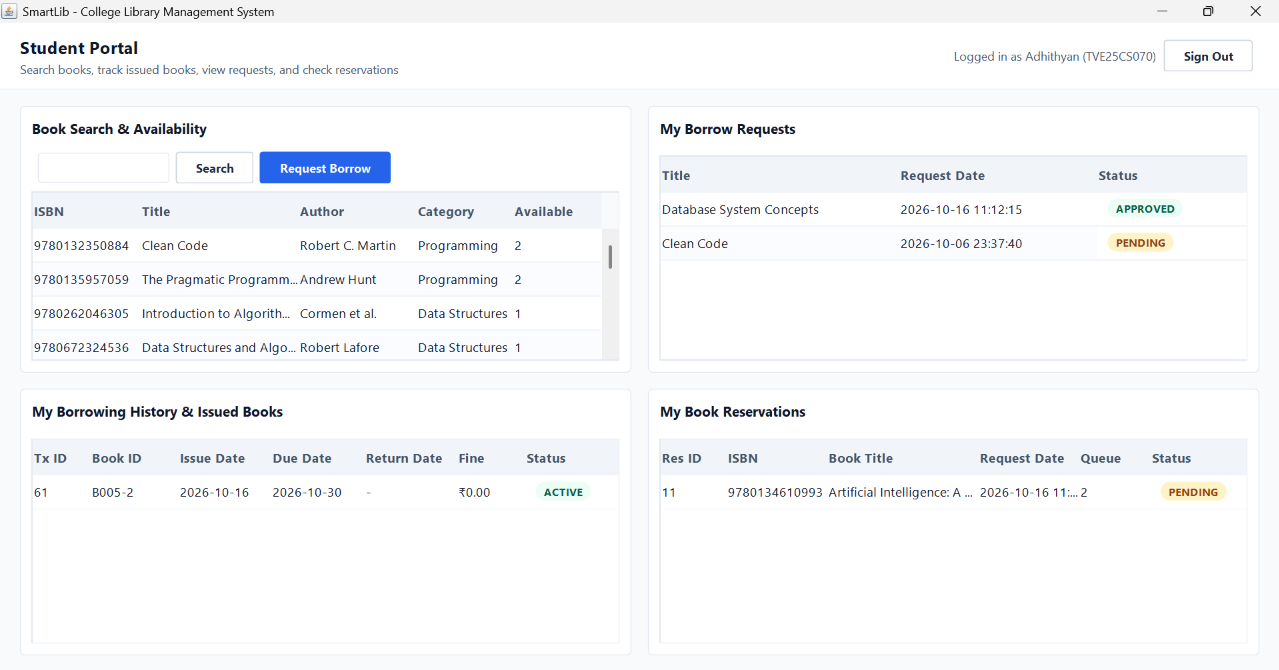
\includegraphics[width=0.94\textwidth]{figures/student-portal.png}
    \caption{Student Self-Service Dashboard (\texttt{StudentDashboardPanel})}
    \label{fig:screenshot_student_dashboard}
\end{figure}

\section{Sample Operational Scenarios and Traces}

To demonstrate system execution, three representative operational workflows are detailed below, tracing user input, service processing, and database state transitions.

\subsection{Scenario A: Direct Book Issue at Circulation Desk}
\begin{itemize}
    \item \textbf{Initial Context:} Book \texttt{"B1001"} (\textit{Effective Java}) is currently on the shelf with status \texttt{AVAILABLE}. Student \texttt{"TVE23CS001"} (\textit{Alice Smith}) presents her college ID card at the desk.
    \item \textbf{Input Data:}
    \begin{itemize}
        \item Student KTU ID: \texttt{"TVE23CS001"}
        \item Book Accession ID: \texttt{"B1001"}
        \item Librarian Session: ID 1 (\texttt{admin})
    \end{itemize}
    \item \textbf{Processing Logic:}
    \begin{enumerate}
        \item \texttt{BorrowService.issueBook()} verifies that \texttt{Student} exists and status is \texttt{ACTIVE}.
        \item Verifies that \texttt{Book.getStatus() == BookStatus.AVAILABLE}.
        \item Generates issue date (\texttt{2026-10-23}) and due date ($\text{Today} + 14 \text{ days} = \text{2026-11-06}$).
        \item Inserts a record into \texttt{borrow\_transactions} with status \texttt{'ACTIVE'}.
        \item Executes \texttt{bookDAO.updateStatus("B1001", BookStatus.ISSUED)}.
    \end{enumerate}
    \item \textbf{Output / Result:} A success dialog displays \textit{"Book issued successfully! Due date: 2026-11-06"}. The book's status pill in the catalog immediately changes from Green (\texttt{AVAILABLE}) to Amber (\texttt{ISSUED}), and the transaction appears in the Active Borrowings table.
\end{itemize}

\subsection{Scenario B: Overdue Book Return with Fine Calculation and Reservation Alert}
\begin{itemize}
    \item \textbf{Initial Context:} Book \texttt{"B1003"} (\textit{Domain-Driven Design}) was issued to \texttt{"TVE23CS001"} with due date \texttt{2023-10-15}. Another student \texttt{"TVE23CS002"} placed a reservation on that ISBN. The book is returned today.
    \item \textbf{Input Data:} Book Accession ID: \texttt{"B1003"}.
    \item \textbf{Processing Logic:}
    \begin{enumerate}
        \item \texttt{BorrowService.returnBook("B1003", 1)} retrieves the active transaction record.
        \item Dynamic fine engine calculates overdue days: $\text{Overdue} = \text{Current Date} - \text{Due Date}$.
        \item Accrued fine computed as $\text{Days Overdue} \times \text{\rupee} 10.00$.
        \item Transaction updated in database: status set to \texttt{'COMPLETED'}, return date set to current date, assessed fine recorded.
        \item Book status reset to \texttt{AVAILABLE}.
        \item \texttt{ReservationDAO.findOldestPendingByIsbn()} detects that a pending reservation exists for \texttt{"TVE23CS002"}.
        \item The service appends an attention notice to the return confirmation message.
    \end{enumerate}
    \item \textbf{Output / Result:} The return is confirmed displaying the fine. An alert dialog informs the librarian: \textit{"ATTENTION: This book is reserved!\textbackslash nNext Student in Queue: TVE23CS002\textbackslash nPlease set this book aside."}
\end{itemize}

\subsection{Scenario C: Student Deletion Safeguard and Audit Protection}
\begin{itemize}
    \item \textbf{Initial Context:} A librarian attempts to delete student record \texttt{"TVE23CS001"} (\textit{Alice Smith}) from the Student Directory desk. The student currently has an active borrowed book and historical loan records.
    \item \textbf{Input Data:} Select row \texttt{"TVE23CS001"} in \texttt{StudentPanel}, click \textit{"Delete Student"}.
    \item \textbf{Processing Logic:}
    \begin{enumerate}
        \item \texttt{StudentService.deleteStudent()} queries the student's associated records across \texttt{BorrowTransactionDAO}, \texttt{BorrowRequestDAO}, and \texttt{ReservationDAO}.
        \item Identifies 1 active borrowed book and associated historical circulation records.
        \item Builds an itemized list of blocking reasons to prevent foreign key errors and preserve historical records.
        \item Throws a descriptive \texttt{LibraryException} instructing the user to deactivate rather than delete.
    \end{enumerate}
    \item \textbf{Output / Result:} An alert dialog appears: \textit{"Cannot permanently delete student TVE23CS001: Related records exist (1 active borrowed book(s)...). To preserve borrowing history, please deactivate the student instead."} The student record remains intact in the database.
\end{itemize}
